\chapter{Stamm- \& Bewegungsdaten}

Die Software unterscheidet zwischen zwei Typen von Umsätzen:

\begin{itemize}[nosep]
	\item Wiederkehrende Umsätze
	\item (Einzigartige) Umsätze
\end{itemize}

\section{Wiederkehrende Umsätze} \label{sec:fixedExpenses}

Wiederkehrende Umsätze treten in einem bestimmten Rhythmus auf (bspw. vierteljährlich oder monatlich) oder aber auch unregelmäßig -- dafür aber wiederkehrend (bspw. Tanken) -- auf.

\begin{figure}[ht!]
	\centering
	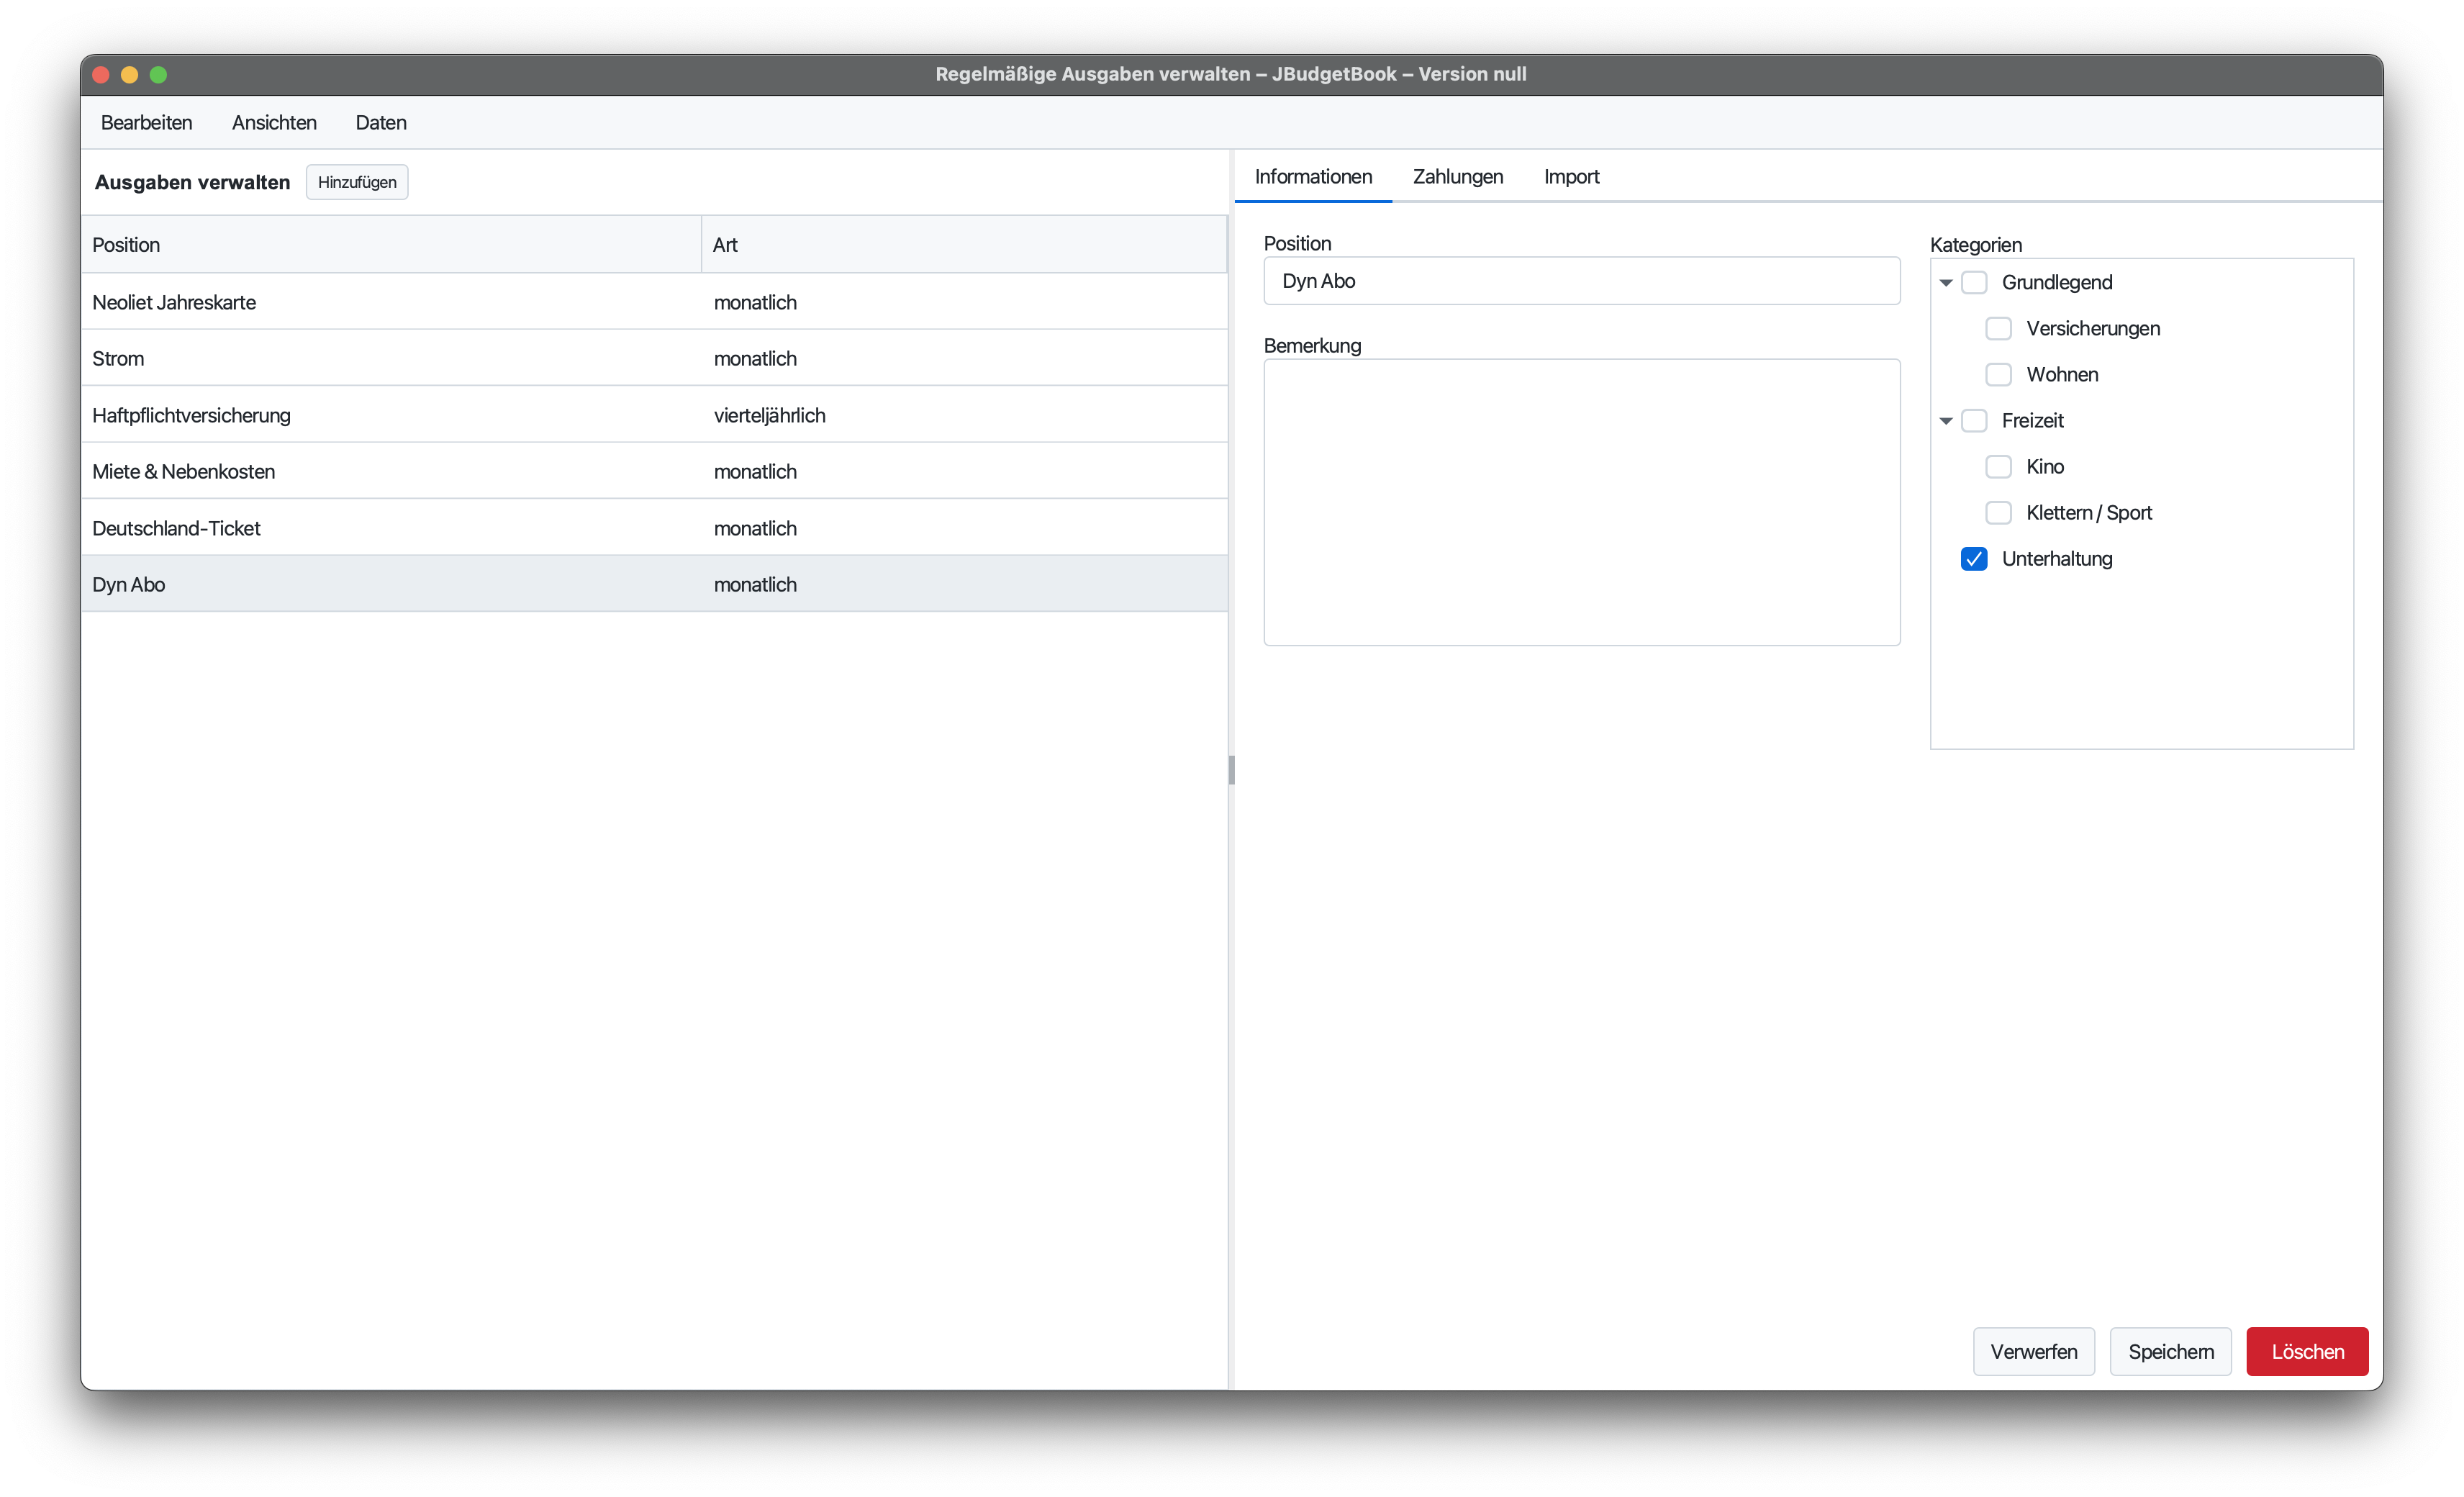
\includegraphics[width=\textwidth]{img/Screenshot-FixedExpenses-MDV}
	\vspace{-2em}
	\caption{Listen- \& Detailansicht der wiederkehrenden Umsätze}
	\label{fig:mdvFixedExpenses}
\end{figure}

In der Detailansicht (s. Abbildung \ref{fig:mdvFixedExpenses} rechts) kann u. a. der Zyklus/Rhythmus (s. "`Zahlungen"' des Umsatzes und die Importregeln festgelegt werden. Beide Angaben sind optional.

\renewcommand{\arraystretch}{1.5}
\begin{table}[!ht]
\centering
\begin{tabular}{|p{6cm}|p{8cm}|}
\hline 
\textbf{Feld} & \textbf{Beschreibung} \\ 
\hline 
Position * & Bezeichnung des Umsatzes \\ 
\hline 
Bemerkung & Anmerkung zum Umsatz \\ 
\hline 
Richtung * & Richtung (Einnahme oder Ausgabe) \\ 
\hline 
Kategorien & Kategorien, denen der Umsatz zugeordnet ist \\ 
\hline 
Zahlungen nur für die Zukunft (und den aktuellen Monat) verwenden & Wenn die Checkbox ausgewählt ist, werden die konfigurierten Zahlungen nicht für die Vergangenheit verwendet (s. Beispiel unten) \\ 
\hline 
\end{tabular} 
\caption{Konfigurationsmöglichkeiten im Tab "`Informationen"'}
\end{table}
\renewcommand{\arraystretch}{1.0}

\renewcommand{\arraystretch}{1.5}
\begin{table}[!ht]
\centering
\begin{tabular}{|p{6cm}|p{8cm}|}
\hline 
\textbf{Feld} & \textbf{Beschreibung} \\ 
\hline 
Betrag * & Höhe des Umsatzes \\ 
\hline 
Art * & Rhythmus des Umsatzes (monatlich, vierteljährlich, halbjährlich, jährlich) \\ 
\hline 
Von * & Bspw. ab wann der Umsatz in dieser Höhe ansteht \\ 
\hline 
Bis & Bspw. bis wann der Umsatz in dieser Höhe ansteht (kann leer gelassen werden, wenn der Umsatz aktuell in dieser Höhe ansteht) \\ 
\hline 
\multicolumn{2}{|p{14cm}|}{In der Tabelle können mehrere "`Zahlungen"' hinterlegt werden. Das ermöglicht die Abbildung von steigenden oder sinkenden Umsätzen, wie es bspw. bei Versicherungsbeiträgen häufig der Fall ist.} \\ 
\hline 
\end{tabular} 
\caption{Konfigurationsmöglichkeiten im Tab "`Zahlungen"'}
\end{table}
\renewcommand{\arraystretch}{1.0}

\renewcommand{\arraystretch}{1.5}
\begin{table}[!ht]
\centering
\begin{tabular}{|p{6cm}|p{8cm}|}
\hline 
\textbf{Feld} & \textbf{Beschreibung} \\ 
\hline 
Tabelle "`Importregeln"' & Diese Tabelle ermöglicht die Verwaltung einer Liste an Importregeln (s. Kapitel \ref{chap:import}) \\ 
\hline 
Tabelle "`Zugeordnete Importe"' & Listet alle zugeordneten Importe auf (readonly) \\ 
\hline 
\end{tabular} 
\caption{Konfigurationsmöglichkeiten im Tab "`Import"'}
\end{table}
\renewcommand{\arraystretch}{1.0}

\begin{infobox}
\textbf{Hinweis zu importierten Umsätzen}: Sollten zu einer Ausgabe reale Umsätze importiert worden sein, werden in den Übersichten (bspw. Monatsansicht) der Betrag dieser importierten Umsätze verwendet und der im System konfigurierte Betrag nur noch als Fallback verwendet. Eine detailliertere Beschreibung findet sich in Kapitel \ref{chap:import}. 
\end{infobox}

Da reale Ausgaben (bzw. Importe) über die Importregeln einer regelmäßigen Ausgabe zugeordnet werden können und dann dieser reale Umsatz in der Software angezeigt wird, können auch wiederkehrende Ausgaben mit schwankenden Beträgen -- wie es beim Tanken der Fall ist -- gruppiert werden.

\subsection*{Beispiel: Tanken}

Die Ausgabe "`Tanken"' soll als wiederkehrender Umsatz (Richtung "`Ausgabe`"') im System abgebildet werden. Dazu kann eine "`Zahlung"' in der Höhe von bspw. 80 Euro monatlich angelegt werden. Allerdings wird nicht jeden Monat getankt, weshalb die Checkbox "`Zahlungen nur für die Zukunft (und den aktuellen Monat) verwenden"' ausgewählt wird. Somit werden bspw. in der Analyseansicht für vergangene Monate die realen Ausgaben angezeigt -- wie sie vom Konto importiert wurden --, während für die Zukunft weiterhin die geplanten Zahlungen aufgeführt werden. Wenn man regelmäßig an einer Star- oder Aral-Tankstelle tankt und mittels Visa-Karte bezahlt, könnten zwei Importregeln konfiguriert werden, die jeweils  "`VISA STAR"' und "`VISA ARAL"' als "`Empfänger enthält"' eingetragen haben. 

Sollte das Import-Feature nicht genutzt werden, kann ein "`realer Umsatz"' auch manuell als (einzigartiger) Umsatz (bzw. Ausgabe) konfiguriert und mit der wiederkehrenden Ausgabe "`Tanken"' verknüpft werden. Dann wird für den entsprechenden Monat ebenfalls der gesamte Betrag dieser Ausgabe verwendet, statt der geplanten Zahlung der wiederkehrenden Ausgabe.


\section{(Einzigartige) Umsätze}

Einzigartige Umsätze treten einmalig oder selten auf, sodass es keinen Mehrwert bietet, diese als regelmäßige Umsätze zu gruppieren (da bspw. keine wiederkehrenden Importe zu Ausgaben dieser Art erwartet werden). Beispiele wären hier der Besuch eines Restaurants oder Ausgaben für Geschenke.

\begin{figure}[ht!]
	\centering
	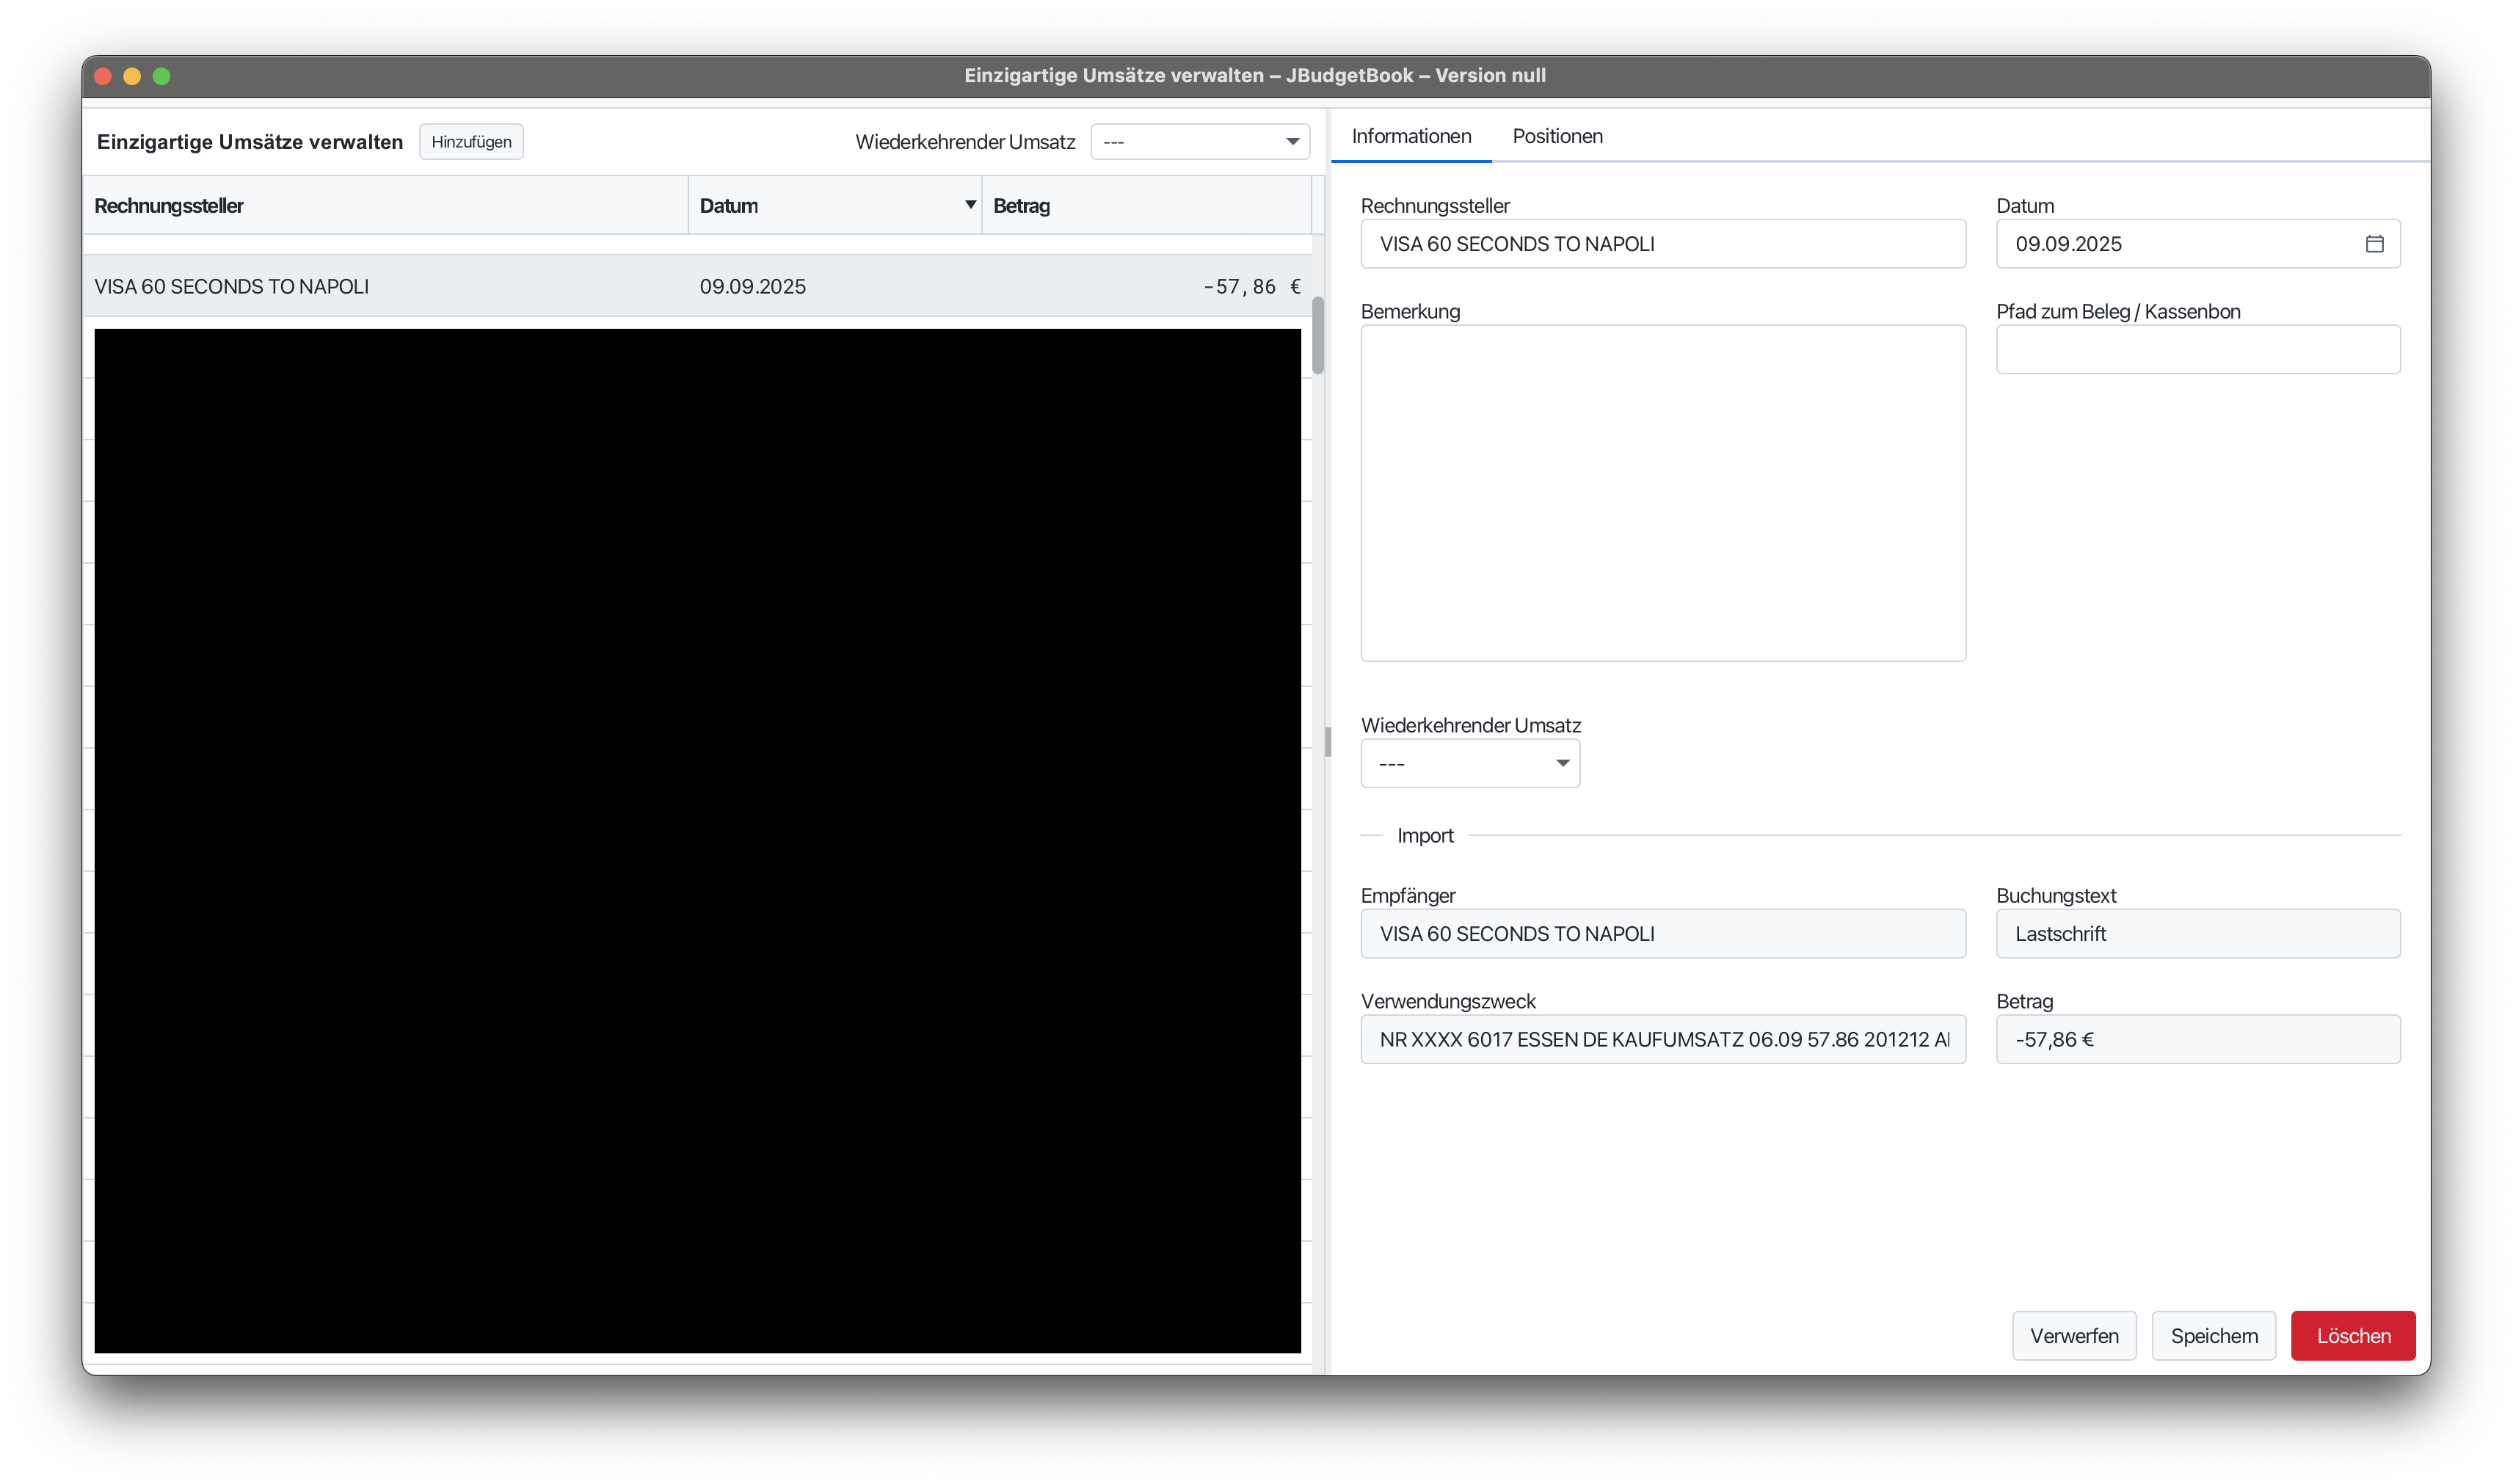
\includegraphics[width=\textwidth]{img/Screenshot-UniqueExpenses-MDV}
	\vspace{-2em}
	\caption{Listen- \& Detailansicht der (einzigartigen) Umsätze}
	\label{fig:mdvFixedExpenses}
\end{figure}

In der Listenansicht werden standardmäßig nur die Umsätze angezeigt, die keinem wiederkehrenden Umsatz zugeordnet sind. Sollen Umsätze angezeigt werden, die wiederkehrenden Umsätzen zugeordnet sind -- und somit den wiederkehrenden Umsatz für den Monat überschreiben --, kann dies über das Dropdown-Menü oben rechts über der Listenansicht erreicht werden.

Die Konfigurationsmöglichkeiten im Tab "`Informationen"' sind in Tabelle \ref{tab:uniqueTurnoverInfoTab} beschrieben. Der Tab "`Positionen"' ermöglicht das hinterlegen einzelner Positionen des Umsatzes, die für sich kategorisiert werden können und ihre eigene Richtung (Einnahme oder Ausgabe) haben. Die Summe dieser Positionen ergibt den Betrag eines (einzigartigen) Umsatzes.

\renewcommand{\arraystretch}{1.5}
\begin{table}[!ht]
\centering
\begin{tabular}{|p{6cm}|p{8cm}|}
\hline 
\textbf{Feld} & \textbf{Beschreibung} \\ 
\hline 
\hline 
\multicolumn{2}{|c|}{Allgemein} \\ 
\hline 
Rechnungsteller * & Rechnungsteller (wird in anderen Ansichten als Name des Umsatzes angezeigt)  \\ 
\hline 
Datum * & Datum des Umsatzes \\ 
\hline 
Bemerkung & Optionaler Kommentar zum Umsatz \\ 
\hline 
Pfad zum Beleg / Kassenbon & Optionaler Dateipfad zum Beleg. Wird als Bild in dieser Ansicht angezeigt \\ 
\hline 
Wiederkehrender Umsatz & Optionaler wiederkehrender Umsatz. Sollte ein wiederkehrender Umsatz ausgewählt sein, wird der Betrag dieses Umsatzes für den Monat verwendet (und nicht der konfigurierte Betrag am wiederkehrenden Umsatz) \\ 
\hline 
\hline 
\multicolumn{2}{|c|}{Import (readonly)} \\ 
\hline 
Empfänger & Empfänger wie er in der Quelle (Konto) des Umsatzes aufgeführt ist \\
\hline
Verwendungszweck & Verwendungszweck wie er in der Quelle (Konto) des Umsatzes aufgeführt ist \\
\hline 
Buchungstext & Art des Umsatzes (bspw. Lastschrift oder Überweisung) wie er in der Quelle (Konto) des Umsatzes aufgeführt ist \\
\hline 
Betrag & Realer Betrag des Umsatzes wie er in der Quelle (Konto) des Umsatzes aufgeführt ist \\
\hline 
\end{tabular} 
\caption{Konfigurationsmöglichkeiten im Tab "`Informationen"'}
\label{tab:uniqueTurnoverInfoTab}
\end{table}
\renewcommand{\arraystretch}{1.0}

\begin{infobox}
\textbf{Hinweis zu importierten Umsätzen}: Für jeden importierten Umsatz wird ein (einzigartiger) Umsatz angelegt, der eventuell einem wiederkehrenden Umsatz zugeordnet ist und den dort konfigurierten Betrag für den Monat überschreibt. Da die Positionen des importieren Umsatzes im System bearbeitet werden können, kann die Summe der Positionen ungleich dem importierten Betrag sein. In dieser Situation wird eine Warnung unterhalb des importierten Betrags angezeigt, aber der konfigurierte Betrag vom System verwendet. 
\end{infobox}

\section{Kategorien und Kategoriegruppen}

Zur Kategorisierung von Umsätzen können Kategorien herangezogen werden, die nochmal zu Gruppen zusammengefasst werden können. An Kategorien kann jeweils ein Budget konfiguriert werden, welches in der Monats- uns Analyseansicht angezeigt wird. 

Die Kategoriegruppen sind aktuell nur als Datenmodell implementiert und finden innerhalb des Systems keine Anwendung in den Ansichten zur Auswertung der Umsätze. 

\section{Datenmodell} 

\begin{figure}[ht!]
	\centering
	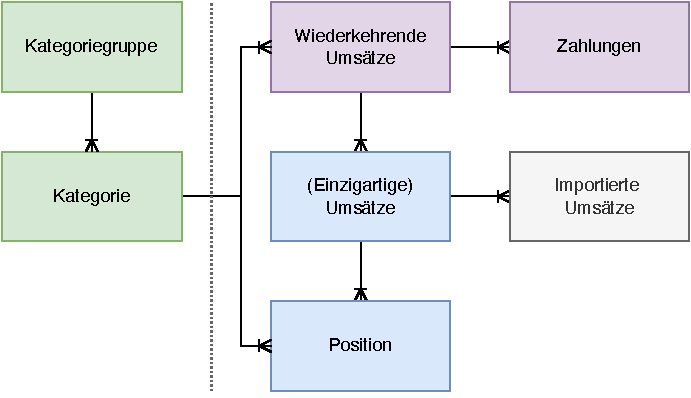
\includegraphics[width=.8\textwidth]{img/DataModel}
	\vspace{0em}
	\caption{Datenmodell}
	\label{fig:datamodel}
\end{figure}

Datenmodel des Systems mit Stammdaten (grün und lila) sowie Bewegungsdaten (blau und grau).